\documentclass{article}
%\usepackage[latin1]{inputenc}
\usepackage{graphicx,amssymb,amsmath,amsbsy,MnSymbol} % extensions pour maths avancées
\usepackage{graphicx,mathenv}           % extensions pour figures
\usepackage[T1]{fontenc}        % pour les charactères accentués 
\usepackage[utf8]{inputenc} 
\usepackage{multicol}
\usepackage{wrapfig}
\usepackage{stmaryrd} % Pour les crochets d'ensemble d'entier
\usepackage{float}  % Pour placer les images là ou JE veux.

\DeclareMathOperator{\tr}{tr}
\DeclareMathOperator{\argmax}{argmax}


\setlength{\parindent}{0.0in}
\setlength{\parskip}{0.1in}
\setlength{\topmargin}{-0.4in}
\setlength{\topskip}{0.7in}    % between header and text
\setlength{\textheight}{9in} % height of main text
\setlength{\textwidth}{6in}    % width of text
\setlength{\oddsidemargin}{0in} % odd page left margin
\setlength{\evensidemargin}{0in} % even page left margin
%
%% Quelques raccourcis clavier :
\def\slantfrac#1#2{\kern.1em^{#1}\kern-.3em/\kern-.1em_{#2}}
\def\b#1{\mathbf{#1}}
\def\bs#1{\boldsymbol{#1}}
\def\m#1{\mathrm{#1}}
\bibliographystyle{plain}
%
\newcommand{\greeksym}[1]{{\usefont{U}{psy}{m}{n}#1}}
\newcommand{\inc}{\mbox{\small\greeksym{d}\hskip 0.05ex}}%
\pagenumbering{arabic}
\date{\today}
\title{Segmentation using MeanShift}
\author{Nelle Varoquaux}
\begin{document}
\maketitle

\begin{abstract}
\textit{Nous présentons ici une étude détaillée de l'algorithme Mean Shift, et
une application à la segmentation de l'image, telle que décrit dans
\cite{my_article}}
\end{abstract}



\section{Introduction}

De nombreuses tâches de vision bas niveau nécessite l'étude d'un espace des
caractéristiques, ou des descripteurs. De nombreuses techniques reposent sur
une bonne évalutation des paramètres: ceux-ci sont souvent devinés. \\
Un espace de paramètres est obtenu en étudiant localement une image: l'image
d'entrée est étudiée par patchs. Des descripteurs sont extraits, et associé à
un point dans l'espace. Une fois que toute l'image est traité, on peut obtenir
les descripteurs les plus significatifs en calculant les régions les plus
denses de l'espace de descripteurs: ces régions correspondent à des clusters.
\\
La nature des descripteurs dépendent de l'application cherchée: cela peut
être des descripteurs locaux à un pixel, telle que une représentation des
couleurs, ou des descripteurs calculés à partir d'un petit patch de l'image,
représentant une texture. \\
L'analyse de cette espace varie elle aussi selon la tâche à effectuer. Malgré
le nombre important d'algorithme de clustering, peu d'entre eux sont adaptés à
l'étude d'un espace de descripteurs: beaucoup reposent sur une
connaissance préalable du nombre de clusters ou de la forme de ceux-ci, ou
alors sont mal adapatés à l'étude d'un espace de descripteurs trop complexe,
ce qui est souvent le cas dans le domaine du traitement d'image. Parmi les
algorithmes de clustering les plus standard, on peut citer le k-means, qui
nécessite une connaissance du nombre de cluster, et les algorithmes
hierarchiques, qui consiste à aggréger des clusters entre eux, ou a les
séparer, trop peu efficace pour le traitement d'image. \\
On présente ici une détection de mode, maxima locaux d'une estimation non
paramétrique de densité de probabilité du noyau.

\section{Mean shift}

\begin{figure}
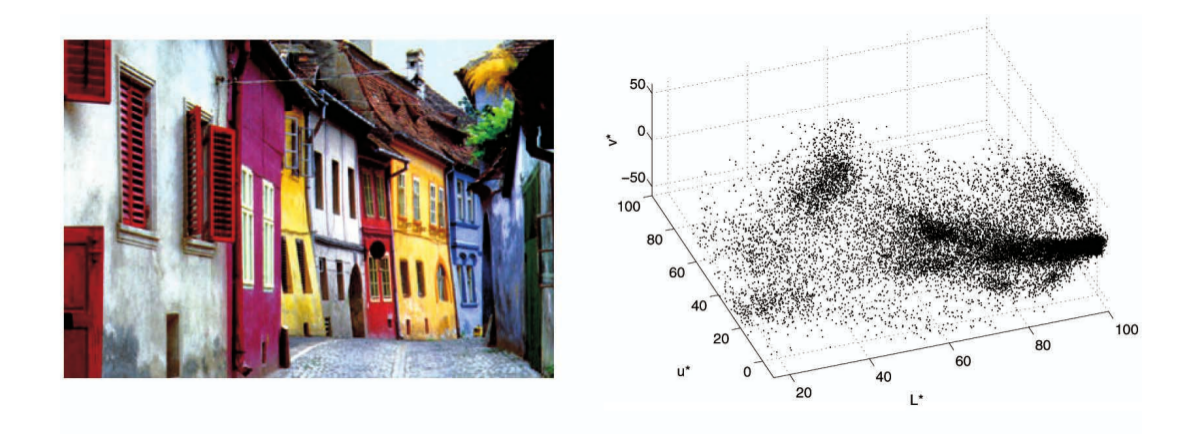
\includegraphics[width=400px]{images/color_space.png}
\end{figure}

L'algorithme de clustering Mean Shift ne nécessite pas la connaissance a
priori du nombre de cluster, ni la forme des clusters. Présenté pour la
première fois par \cite{fukugana} en 1975, le mean shift est un estimateur non
paramétrique du gradient de la densité de probabilité. Peu connu, il est
ensuite généralisé par \cite{cheng} en 1995. Une application au filtrage et à la
segmentation est ensuite proposée en 1997, 1999 dans \cite{comaniciu_meer}. Il est ensuite
utilisé dans des domaines tels que le suivi d'objet, le maillage, et la
segmentation d'image. Cette grande variété d'application s'explique par
l'exploitation de l'espace des descripteurs. \\
L'algorithme repose sur la recherche de maximum d'une densité de probabilité,
\textit{un mode}. Une région est caractérisée par une densité de probabilité,
elle même représentée par un mode. Plusieurs régions impliquent donc plusieurs
modes. Trouver à quelle région appartient une donnée correspond donc à trouver
le mode de cette donnée.

\begin{itemize}
\item Déterminer aléatoirement des régions d'interêt
\item Déterminer les centroïdes des régions
\item Recalculer les régions d'interêt autour des centroïdes
\item Répeter les étapes jusqu'à la convergence
\end{itemize}

\begin{figure}
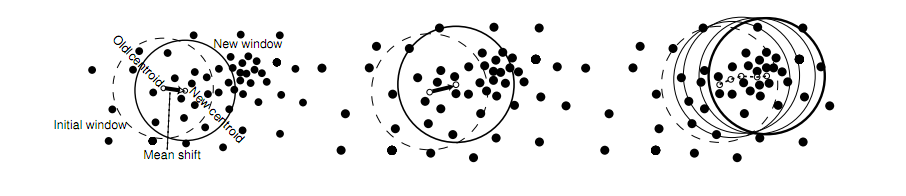
\includegraphics[width=400px]{images/mean_shift_proc.png}
\end{figure}

On note $K(x)$ la fonction à noyaux, qui indique comment $x$ contribut à
l'estimation de la moyenne. On peut alors calculer la moyenne $m$ de $x$:

\begin{equation*}
m(x) = \frac{\sum_{i = 1}^n K (x - x_i) x_i}{\sum_{i = 1}^n K (x - x_i)}
\end{equation*}

On appelle la différence $m(x) - x$ mean shift.

La méthode la plus populaire pour estimer la densité de probabilité est la
technique de la fenêtre de Parzen. Sachant $n$ point $x_i, i = 1, \dots, n$
dans l'espace $R^d$, une bande passante $H$, et un noyau $K(x)$, l'estimateur
de la densité est:

\begin{equation}
\hat{f}(x) = \frac{1}{n} \sum_{i = 1}^n K_H(x - x_i)
\end{equation}

Pour les noyaux à symmétrie circulaire, il suffit de définir le profile du
noyau $k(x)$. On a alors:

\begin{equation}
K(x) = c_{k, d} k (|| x ||^2)
\end{equation}

$x_{k, d}$ est une constante de normalisation strictement positive, permettant
d'assurer la contrainte suivante:

\begin{equation*}
\int_{R^d} K(x) dx = 1
\end{equation*}

Si complétement paramétrisée, la bande passante $H$ permet de raffiner
l'estimation. Elle est cependant souvant choisie comme étant diagonale 
$H = diag [h_1^2, \dots, h_n^2]$, ou proportionnelle à l'identité $H = h \times
I$. Nous nous restreindrons à ce dernier cas, ce qui permet de ne définir
qu'un seul paramètre. Avec cette contrainte supplémentaire, la densité
s'écrit:

\begin{equation}
\hat{f}(x) = \frac{1}{nh^d} \sum_{i = 1}^n K\(\frac{x - x_i}{h}\)
\end{equation}


\begin{figure}
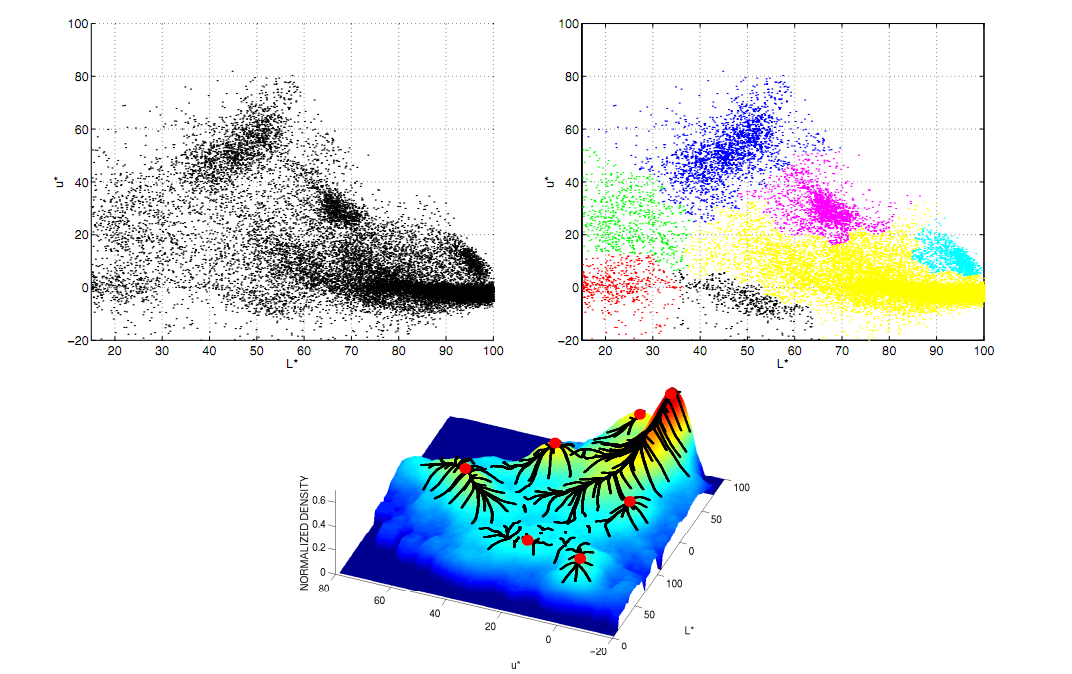
\includegraphics[width=450px]{images/mean_shift_color_space.png}
\end{figure}

\section{Descripteurs pour la segmentation}

Parmi les descripteurs intuitifs d'une image, on peut citer les différents
espaces de couleurs. Des descripteurs de texture peuvent aussi être utilisés,
ainsi qu'une combinaison des descripteurs de couleurs et de texture.

\subsection{Couleurs}

On dispose de plusieurs espaces de couleurs, que nous pouvons utiliser comme
descripteurs:

\begin{itemize}
\item niveau de gris: le descripteurs le plus simple est certainement le
niveau de gris. Étant d'une dimension, le calcul du meanshift est
particulièrement rapide sur celui-ci. Il est d'un interêt limité.
\item RGB: cet espace corresponds aux couleurs primaires, qui correspondent
aux trois longueurs d'onde auxquelles répondent l'oeil humain.
\item HSV (hue saturation value): cet espace de teinte, saturation et valeur,
est obtenu par une transformatio non linéaire de l'espace de couleur RGB
\item XYZ: cet espace se rapproche vers une description des couleurs conforme
à la vision humain, celui introduisant la notion subjective de la luminance.
\end{itemize}

\subsection{Textures}

Il existe plusieurs manières de représenter les textures. Nous nous limiterons
ici aux textures microscopiques: nous ignorerons donc le cas des textures
macroscopiques, dont nous pouvons distinguer les éléments géométriques
(pommes, galets etc...). Il est cependant bon de rappeler qu'une texture
macroscopique peut devenir microscopique avec un changement d'échelle.

Une texture microscopique est très bien représentée par les statistiques de
premier ordre:
\begin{itemize}
\item Moyenne: $\mu(I) = \frac{1}{N^2} \sum_z I(z)$
\item Variance: $\sigma^2(I) = \frac{1}{N^2} \sum_z (I(z) - \mu)$
\item Energie: $E(I) = \frac{1}{N^2} \sum_z (I(z)^2$
\item Entropie: $H(I) = - \sum_{g = 1}^G f(g) \log(f(g))$
\end{itemize}

Ces quantités ne dépendent que de l'histogramme de l'image, et peuvent donc
prendre des valeurs arbitraires sous l'effet d'un changement de constraste.
Ces descripteurs  sont estimés sur des voisinages bornées, avec des patchs
glissants: ils sont donc approximativement liés à une localisation.

\bibliography{biblio}

\end{document}
